\documentclass[11pt]{article}
\usepackage[margin=1.1in]{geometry}
\usepackage{booktabs}
\usepackage{amsmath}
\usepackage{graphicx}
\usepackage{xcolor}
% Paper chrome matches the UK sister paper (PolicyEngine/uk-ai-study):
% template blue for headings and links, PolicyEngine teal in figures.
\definecolor{paperblue}{rgb}{0,0,0.7}
\definecolor{peteal}{HTML}{39C6C0}
\usepackage{sectsty}
\allsectionsfont{\color{paperblue}}
\usepackage[colorlinks=true, citecolor=paperblue, linkcolor=paperblue, urlcolor=paperblue]{hyperref}
\usepackage[hang,flushmargin]{footmisc}
\usepackage{natbib}
\bibliographystyle{apalike}
% values_generated.tex — machine-generated by analysis/emit_paper_values.py
% from analysis/outputs/ai_scenarios.json, src/data/shiftSweepData.json and
% analysis/outputs/yale_publishable_2030.xlsx. DO NOT EDIT BY HAND.
\newcommand{\genBaselinePovertyPct}{12.13}
\newcommand{\genBaselineGini}{0.4678}
\newcommand{\genRapidFixedRev}{+576}
\newcommand{\genRapidPropRev}{+211}
\newcommand{\genRapidExpRev}{+252}
\newcommand{\genRapidCompRev}{+173}
\newcommand{\genRapidShareKeptPct}{37}
\newcommand{\genRapidFixedPovPp}{-1.09}
\newcommand{\genRapidPropPovPp}{+0.11}
\newcommand{\genRapidCompPovPp}{-1.54}
\newcommand{\genRapidExpPovPp}{+1.72}
\newcommand{\genRapidPovSpanPp}{3.26}
\newcommand{\genRapidRevRelMovePct}{46}
\newcommand{\genRapidCompLambda}{0.928}
\newcommand{\genRapidExpLambda}{1.072}
\newcommand{\genRapidCompCrossover}{118,287}
\newcommand{\genRapidExpCrossover}{168,205}
\newcommand{\genSSCap}{214,200}
\newcommand{\genShareWagesAboveCapPct}{15.8}
\newcommand{\genShareWorkersAboveCapPct}{5.7}
\newcommand{\genModelledLaborShareT}{15.9}
\newcommand{\genModelledCapitalShareT}{5.3}
\newcommand{\genRapidCompPayroll}{+34}
\newcommand{\genRapidPropPayroll}{-16}
\newcommand{\genRapidExpPayroll}{-70}
\newcommand{\genRapidCompLaborPct}{-0.94}
\newcommand{\genGrossTaxSwing}{122}
\newcommand{\genTransferSwing}{43}
\newcommand{\genTransferAbsorbPct}{35}
\newcommand{\genBenefitSwing}{28}
\newcommand{\genRapidCompBenefits}{-14}
\newcommand{\genRapidExpBenefits}{+14}
\newcommand{\genSnapSwing}{19}
\newcommand{\genRapidCompSnap}{-9}
\newcommand{\genRapidExpSnap}{+10}
\newcommand{\genSsiSwing}{3}
\newcommand{\genCreditSwing}{15}
\newcommand{\genModCompBenefits}{-8}
\newcommand{\genModExpBenefits}{+6}
\newcommand{\genNetRevSwing}{79}
\newcommand{\genRapidCompState}{+24}
\newcommand{\genRapidPropState}{+36}
\newcommand{\genRapidExpState}{+48}
\newcommand{\genRapidExpStateNet}{+47}
\newcommand{\genStateTopFiveSharePct}{56}
\newcommand{\genStateFirst}{CA +10.0}
\newcommand{\genStateSecond}{NY +5.8}
\newcommand{\genStateThird}{NJ +1.6}
\newcommand{\genStateFourth}{MA +1.3}
\newcommand{\genStateFifth}{MD +1.2}
\newcommand{\genWAState}{+1.1}
\newcommand{\genNZeroStates}{7}
\newcommand{\genZeroStatesList}{Florida, New Hampshire, Nevada, South Dakota, Tennessee, Texas and Wyoming}
\newcommand{\genZeroStatesCodes}{FL, NH, NV, SD, TN, TX, WY}
\newcommand{\genRealZeroRev}{-60}
\newcommand{\genRealFullRev}{+211}
\newcommand{\genRealBreakevenPct}{22.5}
\newcommand{\genRealGridStepPct}{25}
\newcommand{\genRealQuarterRev}{+7}
\newcommand{\genRealPovMinPct}{12.24}
\newcommand{\genRealPovMaxPct}{12.27}
\newcommand{\genRealPovSpanPp}{0.03}
\newcommand{\genTheirRapidCit}{+84}
\newcommand{\genCitWedgeMaxDevB}{0.014}
\newcommand{\genTheirNCells}{18}
\newcommand{\genRealZeroAllIn}{+24}
\newcommand{\genSlowScopeFull}{+6}
\newcommand{\genSlowScopeExcl}{-4}
\newcommand{\genModScopeFull}{+144}
\newcommand{\genModScopeExcl}{+98}
\newcommand{\genRapidScopeFull}{+211}
\newcommand{\genRapidScopeExcl}{+106}
\newcommand{\genRapidScopeDiff}{-105}
\newcommand{\genRapidScopeDiffAbs}{105}
\newcommand{\genRapidPropMarketDelta}{+760}
\newcommand{\genRapidPropATRPct}{27.8}
\newcommand{\genBridgeOursIIT}{+287}
\newcommand{\genBridgeOursPayroll}{-70}
\newcommand{\genBridgeWedge}{+84}
\newcommand{\genBridgeOursTotal}{+301}
\newcommand{\genBridgeTheirsIIT}{+195}
\newcommand{\genBridgeTheirsPayroll}{-63}
\newcommand{\genBridgeTheirsTotal}{+216}
\newcommand{\genBridgeRatio}{1.40}
\newcommand{\genTheirCBORevB}{6,618}
\newcommand{\genBridgeOursCboPct}{4.6}
\newcommand{\genBridgeTheirsCboPct}{3.3}
\newcommand{\genTheirYZeroKT}{4.51}
\newcommand{\genBaseGapPct}{17}
\newcommand{\genIITRatio}{1.47}
\newcommand{\genIITRatioProp}{1.97}
\newcommand{\genPayrollTripletOurs}{+34/-16/-70}
\newcommand{\genPayrollTripletTheirs}{+37/-11/-63}
\newcommand{\genIITGapTriplet}{+93/+95/+91}
\newcommand{\genPayrollMaxCellGap}{6}
\newcommand{\genRapidFixedMarketDelta}{+1519}
\newcommand{\genTiltTheirsSlow}{3.62}
\newcommand{\genTiltOursMatchedSlow}{3.13}
\newcommand{\genTiltOursHouseholdSlow}{7.29}
\newcommand{\genKeptMatchedSlowPct}{32}
\newcommand{\genKeptTheirsSlowPct}{28}
\newcommand{\genKeptHouseholdSlowPct}{14}
\newcommand{\genTiltTheirsMod}{1.71}
\newcommand{\genTiltOursMatchedMod}{1.65}
\newcommand{\genTiltOursHouseholdMod}{1.99}
\newcommand{\genKeptMatchedModPct}{61}
\newcommand{\genKeptTheirsModPct}{59}
\newcommand{\genKeptHouseholdModPct}{50}
\newcommand{\genTiltTheirsRapid}{2.11}
\newcommand{\genTiltOursMatchedRapid}{2.00}
\newcommand{\genTiltOursHouseholdRapid}{2.72}
\newcommand{\genKeptMatchedRapidPct}{50}
\newcommand{\genKeptTheirsRapidPct}{47}
\newcommand{\genKeptHouseholdRapidPct}{37}
\newcommand{\genSlowCompTheirsLowerPct}{84}
\newcommand{\genSlowCompOursLowerPct}{93}
\newcommand{\genSweepYear}{2026}
\newcommand{\genSweepBaseGini}{0.470}
\newcommand{\genSweepFullGini}{0.768}
\newcommand{\genSweepBasePovPct}{13.2}
\newcommand{\genSweepFullPovPct}{61.2}
\newcommand{\genSweepTroughRev}{-880}
\newcommand{\genSweepTroughShift}{90}
\newcommand{\genSweepFullRev}{-790}
\newcommand{\genSweepTenIIT}{+44}
\newcommand{\genSweepTenPayroll}{-147}
\newcommand{\genSweepLaborT}{12.4}
\newcommand{\genSweepCapitalT}{2.7}
\newcommand{\genSweepHHCapSharePct}{51}
\newcommand{\genSweepTopDecilePct}{+58}
\newcommand{\genSweepBottomDecilePct}{+0.8}
\newcommand{\genSweepWorstDecilePct}{-48.5}
\newcommand{\genSweepWorstDecile}{5}
\newcommand{\genForecastShiftSlowPct}{0.9}
\newcommand{\genForecastShiftModPct}{3.1}
\newcommand{\genForecastShiftRapidPct}{7.6}
\newcommand{\genIdentityMaxResidual}{0.000}
\newcommand{\genLaborTargetMaxErr}{$2\times10^{-16}$}
\newcommand{\genModelVersion}{1.764.6}
\newcommand{\genRunnerVersion}{5.0.1}
\newcommand{\genDataBuild}{populace-us-2024-buildp-sparse-rmloss100-cae8640-20260728T011454Z}
\newcommand{\genDataBuildShort}{cae8640}
\newcommand{\genDataBuildDate}{28 July 2026}
\newcommand{\genStabMaxAbsRevB}{5.9}
\newcommand{\genStabMaxRelPct}{12}
\newcommand{\genStabMaxRelModRapidPct}{2.8}
\newcommand{\genStabMaxPovChangePp}{0.11}
\newcommand{\genStabTopOneOld}{8.77}
\newcommand{\genStabTopOneNew}{9.00}
\newcommand{\genBaselineTopOnePct}{9.06}
\newcommand{\genStabNYOld}{3.8}
\newcommand{\genStabNYNew}{5.8}
\newcommand{\genCorrMaxRevMoveB}{8}
\newcommand{\genPubTransferSwing}{57}
\newcommand{\genPubTransferAbsorbPct}{47}
\newcommand{\genPubBaselineGini}{0.4625}
\newcommand{\genPubEarlyHeadStartB}{124}
\newcommand{\genPubHeadStartB}{5}
 % machine-generated numeric macros from run outputs
% tables_generated.tex — machine-generated by analysis/emit_paper_values.py.
% DO NOT EDIT BY HAND.
\newcommand{\tabScenarioGrid}{%
\begin{tabular}{lrrrrrrr}
\toprule
Scenario & Revenue & Income tax & Payroll & State & Poverty & $\Delta$pp & Net Gini \\
\midrule
Slow / shares fixed & +47 & +29 & +10 & +6 & 11.99\% & -0.14 & 0.4680 \\
Slow / compressive & +3 & +3 & -1 & +1 & 12.01\% & -0.12 & 0.4675 \\
Slow / proportional & +6 & +11 & -5 & +2 & 12.17\% & +0.04 & 0.4685 \\
Slow / expansive & +10 & +19 & -10 & +3 & 12.33\% & +0.20 & 0.4695 \\
\addlinespace
Moderate / shares fixed & +287 & +178 & +61 & +35 & 11.46\% & -0.67 & 0.4690 \\
Moderate / compressive & +125 & +65 & +33 & +15 & 11.18\% & -0.95 & 0.4646 \\
Moderate / proportional & +144 & +114 & +7 & +21 & 12.00\% & -0.13 & 0.4709 \\
Moderate / expansive & +165 & +164 & -20 & +28 & 12.84\% & +0.71 & 0.4771 \\
\addlinespace
Rapid / shares fixed & +576 & +358 & +121 & +71 & 11.04\% & -1.09 & 0.4703 \\
Rapid / compressive & +173 & +98 & +34 & +24 & 10.59\% & -1.54 & 0.4630 \\
Rapid / proportional & +211 & +193 & -16 & +36 & 12.24\% & +0.11 & 0.4750 \\
Rapid / expansive & +252 & +294 & -70 & +48 & 13.85\% & +1.72 & 0.4875 \\
\bottomrule
\end{tabular}}
\newcommand{\tabTilt}{%
\begin{tabular}{lrrr}
\toprule
Scenario & Shares fixed & As forecast & Share kept \\
\midrule
Slow & +47 & +6 & 14\% \\
Moderate & +287 & +144 & 50\% \\
Rapid & +576 & +211 & 37\% \\
\bottomrule
\end{tabular}}
\newcommand{\tabRealization}{%
\begin{tabular}{lr}
\toprule
Realized share & Revenue \\
\midrule
0\% & -60 \\
25\% & +7 \\
50\% & +74 \\
75\% & +142 \\
100\% (their assumption) & +211 \\
\bottomrule
\end{tabular}}
\newcommand{\tabCapitalScope}{%
\begin{tabular}{lrrr}
\toprule
Scenario & Full capital set & Excl.\ retirement & Difference \\
\midrule
Slow & +6 & -4 & -10 \\
Moderate & +144 & +98 & -46 \\
Rapid & +211 & +106 & -105 \\
\bottomrule
\end{tabular}}
\newcommand{\tabBridge}{%
\begin{tabular}{lrrrr}
\toprule
Rapid / expansive & IIT (net) & Payroll & Corporate wedge & Total \\
\midrule
This paper & +287 & -70 & +84 & +301 \\
Budget Lab & +195 & -63 & +84 & +216 \\
\bottomrule
\end{tabular}}
\newcommand{\tabPayrollCells}{%
\begin{tabular}{lrrrr}
\toprule
Cell & \multicolumn{2}{c}{IIT net of credits} & \multicolumn{2}{c}{Payroll} \\
 & Ours & Theirs & Ours & Theirs \\
\midrule
Slow / compressive & +3 & -4 & -1 & +0 \\
Slow / proportional & +11 & +4 & -5 & -4 \\
Slow / expansive & +18 & +11 & -10 & -8 \\
\addlinespace
Moderate / compressive & +69 & +18 & +33 & +30 \\
Moderate / proportional & +114 & +64 & +7 & +5 \\
Moderate / expansive & +161 & +111 & -20 & -21 \\
\addlinespace
Rapid / compressive & +104 & +11 & +34 & +37 \\
Rapid / proportional & +193 & +98 & -16 & -11 \\
Rapid / expansive & +287 & +195 & -70 & -63 \\
\bottomrule
\end{tabular}}
\newcommand{\tabStates}{%
\begin{tabular}{lr}
\toprule
State & Net revenue change \\
\midrule
CA & +10.01 \\
NY & +5.82 \\
NJ & +1.58 \\
MA & +1.33 \\
MD & +1.16 \\
VA & +1.15 \\
WA & +1.13 \\
MN & +1.02 \\
IL & +0.91 \\
OR & +0.89 \\
\addlinespace
\multicolumn{2}{l}{\footnotesize 7 states collect exactly \$0: FL, NH, NV, SD, TN, TX, WY.} \\
\bottomrule
\end{tabular}}
\newcommand{\tabSweep}{%
\begin{tabular}{rrrrr}
\toprule
Shift & Revenue & Income tax & Poverty & Net Gini \\
\midrule
0\% & +0 & +0 & 13.2\% & 0.470 \\
10\% & -135 & +44 & 15.0\% & 0.490 \\
20\% & -255 & +101 & 16.9\% & 0.513 \\
30\% & -370 & +176 & 20.1\% & 0.536 \\
40\% & -486 & +265 & 23.9\% & 0.561 \\
50\% & -592 & +371 & 29.3\% & 0.588 \\
60\% & -688 & +493 & 35.4\% & 0.617 \\
70\% & -773 & +638 & 43.1\% & 0.647 \\
80\% & -847 & +807 & 50.7\% & 0.681 \\
90\% & -880 & +1000 & 57.6\% & 0.719 \\
100\% & -790 & +1235 & 61.2\% & 0.768 \\
\bottomrule
\end{tabular}}
 % machine-generated tables from run outputs

\title{\bfseries What if income shifts from labor to capital?\\[0.15cm]
The fiscal and distributional incidence of AI-driven growth in the United
States\thanks{\textbf{Acknowledgements:} the cell-level reconciliation in
Section~\ref{sec:reconciliation} is possible because the Budget Lab at Yale
publishes its code and complete result grids alongside its reports; I thank
them for that practice. All errors are mine. An interactive companion to this
paper is at
\href{https://policyengine.org/us/ai-inequality/income-shift}{policyengine.org/us/ai-inequality/income-shift};
code and data references are in Appendix~\ref{app:repro}.}\\[0.7cm]}
\author{Max Ghenis\thanks{PolicyEngine. Email:
\href{mailto:max@policyengine.org}{max@policyengine.org}.}}
\date{\small \ifcase\month\or January\or February\or March\or April\or May\or
June\or July\or August\or September\or October\or November\or December\fi\
\the\year}

\begin{document}
\maketitle

\begin{abstract}
\noindent I study how AI-driven growth would move United States government
revenue, benefit outlays, poverty and inequality, by running two experiment
families through PolicyEngine-US, an open-source static microsimulation of the
full federal and state tax and transfer system, on openly published microdata.
A mechanism sweep shifts 0--100\% of labor income into capital income under
current law; a scenario set adopts the Budget Lab's calibration of the
\citet{karger2026} forecaster survey --- Slow, Moderate and Rapid adoption
crossed with three wage-inequality variants --- so that remaining differences
between the two models are differences in coverage, not assumptions. In Rapid,
the forecast tilt toward capital keeps \genKeptMatchedRapidPct\% of the
revenue gain that shares-fixed growth would deliver on the federal basis
comparable to the Budget Lab's (they get \genKeptTheirsRapidPct\%), and
\genKeptHouseholdRapidPct\% on the all-government household basis, which
adds states and transfers but has no corporate wedge
(\genRapidPropRev B against \genRapidFixedRev B); it also turns growth's
poverty gain into a marginal loss (\genRapidFixedPovPp pp becomes
\genRapidPropPovPp pp). Across the wage-inequality variants, net revenue
stays within \genRapidCompRev B--\genRapidExpRev B while the poverty outcome
flips sign, from \genRapidCompPovPp pp to \genRapidExpPovPp pp; automatic
transfer responses absorb \genTransferAbsorbPct\% of the gross-tax swing
across those variants, \$\genBenefitSwing B of it in programs outside a
tax-only model, and state tax doubles from \genRapidCompState B to
\genRapidExpState B. Below a realized share of roughly
\genRealBreakevenPct\% of the incremental capital income, the household
sector loses revenue on Rapid AI growth. Reconciled cell by cell against the
Budget Lab's published grid, payroll responses agree in all nine as-forecast
cells to within \$\genPayrollMaxCellGap B, while the bridged headline is
\genBridgeOursTotal B against their \genBridgeTheirsTotal B
(\genBridgeRatio$\times$), concentrated in the income-tax response to the
capital shock.
\end{abstract}

\medskip
\noindent\textbf{Keywords:} artificial intelligence, factor shares,
microsimulation, taxation, transfers, poverty, inequality, state taxes

\medskip
\noindent\textbf{JEL codes:} H24, H53, H71, D31, I32, O33, C63

\newpage
\noindent\textbf{Correction (September 2026).} Earlier versions of this paper
counted Head Start and Early Head Start in household net income.
policyengine-us \genModelVersion{} values both programs at their per-enrollee
cost. The microdata carry a modeled Head Start take-up flag but none for
Early Head Start, so every eligible child under three and every eligible pregnant person counted
as enrolled in Early Head Start. That put \$\genPubEarlyHeadStartB B of Early
Head Start and \$\genPubHeadStartB B of Head Start in 2030 baseline net income,
rising and falling with the wage shocks because eligibility is income-tested.
This version reruns every calibrated scenario on the same model
and data with both programs kept out of net income, as current PolicyEngine
does. Neither program counts toward SPM resources, so the poverty results are
unchanged. Every tax cell is also unchanged. Net revenue cells move by at most
\$\genCorrMaxRevMoveB B, net Gini levels rise by about 0.005 (baseline
\genPubBaselineGini{} to \genBaselineGini{}), and transfers absorb
\genTransferAbsorbPct\% of the Rapid gross-tax swing (\$\genTransferSwing B),
where earlier versions reported \genPubTransferAbsorbPct\%
(\$\genPubTransferSwing B). The mechanism sweep of Section~\ref{sec:sweep} has
not been rerun and still counts both programs in benefit outlays and net
income. This version also corrects the explanation of why the household
keep-rate sits below the federal one: the gap is mainly the Budget Lab's
corporate wedge on the federal basis, not state taxes and transfers
(Section~\ref{sec:reconciliation}).

\medskip
\section{Introduction}\label{sec:intro}

Forecasters expect artificial intelligence to raise output and, at the same
time, to tilt its composition away from labor and toward capital
\citep{karger2026}. The United States taxes those two kinds of income very
differently, and it runs a transfer system that responds automatically when
wages fall. So the fiscal and household consequences of AI-driven growth
depend not mainly on how much growth arrives, but on which incomes it arrives
in --- and on which parts of the fiscal system a model can see. The Budget
Lab at Yale recently scored AI growth scenarios through a federal individual
income and payroll tax microsimulation and found that a growing capital share
mutes the revenue gains \citep{iselinnunn2026}. Their model, by design, stops
at the tax code: no transfer programs beyond tax credits, no poverty
measurement, no state systems.

This paper runs the same question through the whole system. PolicyEngine-US
is an open-source static microsimulation of United States federal and state
tax and benefit law --- income and payroll taxes, refundable credits, SNAP,
SSI, TANF, WIC and the other major transfer programs, and the Supplemental
Poverty Measure (SPM) --- running on openly published microdata. I use it in
two complementary designs. The first is a mechanism sweep: shift 0--100\% of
positive labor income into capital income, holding modelled market income
fixed, and record what current law does at each step. The second is a
calibrated scenario set that deliberately adopts the Budget Lab's
implementation of the \citet{karger2026} forecaster survey --- Slow, Moderate
and Rapid adoption paths crossed with compressive, proportional and expansive
wage-inequality variants, plus their shares-fixed counterfactuals --- so that
where the two models differ, the difference is model coverage rather than
scenario assumptions. Because they publish their code and their complete
result grid, the comparison can then be made cell by cell on an identical
accounting basis.

Four findings organize the paper. First, the composition tilt, not the growth
rate, drives the fiscal and poverty results. Rapid adoption with factor
shares held at today's levels raises net government revenue by
\genRapidFixedRev B in 2030 and cuts SPM poverty by
\genRapidFixedPovPp pp; the same growth with the forecast tilt keeps
\genKeptHouseholdRapidPct\% of that revenue (\genRapidPropRev B) and turns
the poverty gain into a marginal loss (\genRapidPropPovPp pp). The keep-rate
is basis-dependent, and the paper reports it both ways: on the narrower
federal basis that the Budget Lab measures, the tilt keeps
\genKeptMatchedRapidPct\% here and \genKeptTheirsRapidPct\% in their grid.
The household figure is lower mainly because that basis has no corporate
wedge, which grows with the capital shock; adding state taxes and the
transfer system raises the tilt's dollar cost but barely moves the keep-rate.

Second, the assumption with the least evidence behind it --- whether AI
compresses or widens the wage distribution, a question the forecaster survey
does not elicit and the Budget Lab spans with stylized variants --- decides
the household verdict while leaving the revenue verdict intact. Across the Budget Lab's own
compressive-to-expansive span, Rapid net revenue stays between
\genRapidCompRev B and \genRapidExpRev B, always positive, while the poverty
outcome flips sign: \genRapidCompPovPp pp under compression,
\genRapidExpPovPp pp under expansion, a \genRapidPovSpanPp pp span.

Third, the parts of the fiscal system outside a tax-only model respond
materially, and in both directions. Across those same wage-spread variants,
gross tax collections swing \$\genGrossTaxSwing B, and automatic transfer
responses absorb \genTransferAbsorbPct\% of that swing ---
\$\genBenefitSwing B of it in non-credit programs such as SNAP and SSI that a
tax microsimulation does not carry. State tax codes add
\genRapidPropState B under proportional Rapid growth and double across the
variants, from \genRapidCompState B to \genRapidExpState B. Whether these
channels matter is exactly the kind of question a full-system model exists to
answer.

Fourth, two definitional choices about the tax base move the revenue answer
by more than the choice between Slow, Moderate and Rapid. If AI's incremental
capital income goes unrealized --- retained, accrued, or sheltered inside
retirement accounts --- revenue falls roughly linearly, and below a realized
share of roughly \genRealBreakevenPct\% the household sector loses money on
Rapid AI growth; poverty, meanwhile, moves by
\genRealPovSpanPp~pp across the whole sweep. And whether
taxable retirement distributions count as capital income halves the Rapid
estimate when excluded (\genRapidScopeFull B to \genRapidScopeExcl B).

The reconciliation with the Budget Lab in Section~\ref{sec:reconciliation} is,
to my knowledge, the first cell-level comparison of two independent
microsimulations of AI fiscal scenarios. It is reassuring where the models
share machinery --- payroll responses agree in all nine cells to within
\$\genPayrollMaxCellGap B, two independent wage distributions meeting the
same taxable maximum --- and
informative where they do not: the bridged headline is \genBridgeOursTotal B
against their \genBridgeTheirsTotal B (\genBridgeRatio$\times$), with the gap
concentrated in the income-tax response to the capital shock --- nearly
constant in absolute terms across the wage-spread cells --- consistent with
this paper's \genBaseGapPct\% larger realized-capital base and more
top-concentrated allocation rule.

The paper proceeds as follows. Section~\ref{sec:literature} places the
exercise in the literature. Section~\ref{sec:method} describes the model,
data, and both experiment designs. Section~\ref{sec:results} reports the
sweep and scenario results, including the transfer-system and state channels.
Section~\ref{sec:sensitivity} reports the realization and capital-scope
sensitivities and stability across data builds.
Section~\ref{sec:reconciliation} reconciles with the Budget Lab cell by cell.
Section~\ref{sec:discussion} discusses limitations and next steps.

\input{sections/literature}
\section{Model, data, and experiment designs}\label{sec:method}

\subsection{Model and data}

All results come from PolicyEngine-US version \genModelVersion{}
\citep{policyengineus}, an open-source static microsimulation of United
States federal and state tax and benefit law, executed through the
\texttt{policyengine.py} runtime (version \genRunnerVersion{}), which
certifies the pairing of model version and dataset build. The 2030 baseline
is current law as of that model version, including the 2025 reconciliation
act. The dataset is \texttt{populace-us} build \texttt{\genDataBuildShort}
(\genDataBuildDate{}) \citep{populaceus}, an openly published enhanced-CPS
microdata file for 2024, uprated by the model to the analysis years; scenario
growth is defined in excess of the CBO baseline path, which is exactly right
only where the model's own uprating tracks CBO's projection. The mechanism
sweep of Section~\ref{sec:sweep} is run at \genSweepYear{}; the calibrated
scenarios are run at 2030, matching the Budget Lab's horizon. In the 2030
baseline, SPM poverty is \genBaselinePovertyPct\% and the household
net-income Gini is \genBaselineGini{} (household-level, unequivalized;
Section~\ref{sec:discussion} discusses comparability).

The model covers federal individual income tax (including capital gains
rates, the net investment income tax and the alternative minimum tax),
payroll taxes on both employee and employer sides plus self-employment tax,
refundable credits (EITC, refundable CTC and others), the major means-tested
transfer programs (SNAP, SSI, TANF, WIC, school meals, housing subsidies,
broadband subsidies), and the tax and benefit codes of all fifty states and
DC. Health programs (Medicaid, CHIP, ACA subsidies) are valued in the model
but excluded from net-income accounting in these runs by the model's default
simulation switch, so no result here contains a health-program response in
either direction. Head Start and Early Head Start are likewise valued in the
model but kept out of net income in the calibrated scenarios, as current
PolicyEngine does. The mechanism sweep predates that correction and still
counts both programs in benefit outlays and net income (see the correction
before the introduction). Everything is static: no labor supply, behavioral,
avoidance or enforcement responses, matching the Budget Lab's individual
microsimulation.

\textbf{Accounting.} Net government revenue is defined as taxes minus
transfers: household tax before refundable credits (federal and state,
including employee-side payroll) plus employer payroll tax, minus refundable
credits and benefit outlays. An identity check --- the change in market
income minus the change in household net income must equal the household-side
revenue change --- closes to within \$0.001B in every scenario (maximum
absolute residual \$\genIdentityMaxResidual B at three decimals).
Where the paper compares against the Budget Lab
(Section~\ref{sec:reconciliation}), it restates results on their narrower
basis: federal individual income tax net of refundable credits, plus payroll.

\subsection{Design I: the mechanism sweep}\label{sec:method-sweep}

The sweep isolates composition. In 10-point steps from 0\% to 100\%, it
reduces every person's positive employment and self-employment income by the
step share and redistributes the same weighted total to positive capital
income in proportion to existing holdings, holding modelled market income
fixed. Capital income here means the six directly held flows (long- and
short-term capital gains, taxable interest, qualified and non-qualified
dividends, and rental income); the calibrated scenarios of
Section~\ref{sec:method-scenarios} use a wider nine-variable set that adds
pass-through and taxable retirement income, which is why the two baselines'
capital aggregates differ. The \genSweepYear{} sweep baseline contains
\$\genSweepLaborT T of positive labor income and \$\genSweepCapitalT T of
positive capital income on the six-variable definition, with
\genSweepHHCapSharePct\% of households receiving any positive capital income
--- so the sweep concentrates income by construction, and the question is
what current law does about it.

The sweep's limitation is deliberate: a pure reallocation holds output fixed,
while forecasters expect AI to raise output \emph{and} tilt its composition.
The sweep therefore answers ``what does composition alone do to current
law?'', and the calibrated scenarios answer ``what happens on the paths
forecasters actually expect?''. The two connect through a
forecast-equivalence mapping: the proportional reduction in labor's income
share that each tilt produces, $k = 1 - (1+g_L)/(1+g_Y)$, is also the sweep
position delivering the same share reduction, placing the scenarios at
\genForecastShiftSlowPct\% (Slow), \genForecastShiftModPct\% (Moderate) and
\genForecastShiftRapidPct\% (Rapid) --- the sweep's forecast-relevant range
is its first decade, and the rest is out-of-sample stress test.

\subsection{Design II: forecaster-calibrated scenarios}\label{sec:method-scenarios}

The scenarios adopt the Budget Lab's calibration of \citet{karger2026}
exactly. Each scenario is defined by an annual real GDP growth rate under AI
(Slow 2.0\%, Moderate 2.6\%, Rapid 3.3\%) and a 2030 labor share of factor
income (55.0\%, 53.8\%, 51.3\%). Growth is expressed in excess of the CBO
baseline path: the five-year output shock is
$g_Y = (1+r_{\mathrm{ai}})^5 / G_{\mathrm{CBO}} - 1$, and the factor shocks
follow from the target shares,
\begin{equation}
g_K = \frac{\theta^1_K (1+g_Y) - \theta^0_K}{\theta^0_K}, \qquad
g_L = \frac{\theta^1_L (1+g_Y) - \theta^0_L}{\theta^0_L}.
\end{equation}
Two inputs their report uses but does not print --- the cumulative CBO
baseline factor $G_{\mathrm{CBO}} = 1.0976$ and the pre-shock labor share
$\theta^0_L = 0.5550$ --- are recovered by inverting their published
formulas against the nine derived values in their Table~1; unit tests
reproduce all nine to within 0.005\,pp and re-derive the labor share by grid
search so the constants cannot drift.

The wage-inequality channel is their stylization $\lambda = 1 \pm g_Y$: a
spread transform on log labor income,
$\ln Y^1_i = \mu^1 + \lambda\,(\ln Y^0_i - \mu^0)$, equivalently
$Y^1_i = C\,Y_i^{0\,\lambda}$ with $C$ in closed form, with the aggregate
pinned to $(1+g_L)$ times baseline. Compressive ($\lambda<1$) narrows the
wage distribution around the same aggregate; expansive ($\lambda>1$) widens
it; proportional scales every wage equally. The transform is applied at the
person level because the payroll result turns on a per-person threshold, the
Social Security taxable maximum (\$\genSSCap{} in 2030; at baseline
\genShareWagesAboveCapPct\% of wage income and
\genShareWorkersAboveCapPct\% of workers sit above it).

The capital shock scales nine capital income variables --- long- and
short-term capital gains, taxable interest, qualified and non-qualified
dividends, rental income, partnership and S-corporation income, taxable
pension income and taxable IRA distributions --- in proportion to existing
holdings, after routing pass-through income through the Budget Lab's
labor/capital split rule. The wage-spread transform is not applied to the
labor portion of pass-through income, which follows the pass-through rule
instead. Appendix~\ref{app:routing} traces every shocked
variable into IRS gross income and household market income, confirming the
shock reaches the tax base rather than being recomputed away; the labor
aggregate lands on its target to within relative error
\genLaborTargetMaxErr{}. Each scenario also has a shares-fixed
counterfactual growing both factors at $g_Y$, the comparison behind the
Budget Lab's ``roughly twice as large'' finding.

Two further axes vary definitional assumptions their report flags. A
\emph{realization rate} routes a fraction of the incremental capital flow
outside the taxable base (their assumption corresponds to 1.0); and a
\emph{capital-scope} variant excludes taxable pension income and IRA
distributions from the capital set, since those are taxed at ordinary rates
and their inclusion works against the ``capital is taxed lightly''
mechanism.

\section{Results}\label{sec:results}

\subsection{The mechanism at full range}\label{sec:sweep}

Figure~\ref{fig:sweep-rev} runs the composition mechanism from 0\% to 100\%.
Net government revenue falls almost monotonically as labor income becomes
capital income, bottoming at \genSweepTroughRev B at a
\genSweepTroughShift\% shift. The decomposition is not what a
``capital-is-taxed-lightly'' intuition alone would predict: the federal
income tax \emph{gains} at every step (\genSweepTenIIT B at the first),
because concentrating income into the small capital-holding population
pushes it into upper brackets by more than the preferential rates give back.
Revenue falls anyway because payroll collections fall roughly linearly with
the wage base (\genSweepTenPayroll B at the first step) and benefit outlays
and refundable
credits rise as wage-dependent households qualify for means-tested support;
state codes track the federal income-tax pattern.
The distributional counterpart (Figure~\ref{fig:sweep-dist}) is severe by
construction --- only \genSweepHHCapSharePct\% of households hold any
positive capital income, so the net-income Gini rises from
\genSweepBaseGini{} to \genSweepFullGini{} and SPM poverty from
\genSweepBasePovPct\% to \genSweepFullPovPct\% at the full shift, with the
top decile's mean net income rising \genSweepTopDecilePct\% while decile
\genSweepWorstDecile{} falls \genSweepWorstDecilePct\%. The exception is
instructive and is the transfer system's signature: the bottom decile ends
essentially where it started (\genSweepBottomDecilePct\%), because its income
is largely transfers, which do not follow wages out of the labor market. The
forecast-equivalent range --- the shaded band at
\genForecastShiftSlowPct{}--\genForecastShiftRapidPct\% --- says how much of
this axis the 2030 forecasts actually reach: the first decade. The sweep's
value is the mechanism it exposes, not the tail. These sweep runs predate the
correction noted before the introduction: their benefit outlays and net
income still include Head Start and Early Head Start.

\begin{figure}[t]
\centering
\includegraphics[width=0.92\textwidth]{figures/sweep_revenue.pdf}
\caption{Revenue under a 0--100\% labor-to-capital shift,
\genSweepYear{}. Lines are changes against baseline; benefit outlays are
sign-flipped so a rising line is a fiscal cost. The shaded band marks the
forecast-equivalent positions of the 2030 scenarios.}
\label{fig:sweep-rev}
\end{figure}

\begin{figure}[t]
\centering
\includegraphics[width=0.92\textwidth]{figures/sweep_distribution.pdf}
\caption{Inequality and poverty under the same sweep.}
\label{fig:sweep-dist}
\end{figure}

\subsection{Calibrated scenarios}\label{sec:scenarios}

Table~\ref{tab:grid} reports all twelve scenario cells at 2030 against the
same-year current-law baseline; Figure~\ref{fig:scenarios} plots the Rapid
pattern. Two published Budget Lab mechanisms reproduce on independent
machinery. Within each scenario, moving from compressive to expansive raises
income-tax revenue through progressivity and lowers payroll revenue as
earnings cross the Social Security taxable maximum. And the tilt is
expensive: Table~\ref{tab:tilt} shows each scenario keeping a fraction of its
shares-fixed revenue --- \genKeptHouseholdRapidPct\% in Rapid
(\genRapidPropRev B against \genRapidFixedRev B) on this all-government
household basis, against \genKeptMatchedRapidPct\% on the narrower federal
basis Section~\ref{sec:reconciliation} matches to the Budget Lab. The
difference between those two keep-rates is mainly the Budget Lab's corporate
wedge, which the federal basis includes: it grows with the capital shock, so
it cushions the as-forecast cell. The state and transfer channels add to the
tilt's dollar cost but leave the keep-rate essentially unchanged.

\begin{table}[t]
\centering
\small
\tabScenarioGrid
\caption{Scenario grid, 2030, \$B change against the current-law baseline
(SPM poverty \genBaselinePovertyPct\%, net Gini \genBaselineGini{}).
``Revenue'' is net government revenue (federal and state taxes minus
refundable credits and benefits); ``Income tax'' is federal income tax
gross of refundable credits; ``State'' is state tax before refundable state
credits.}
\label{tab:grid}
\end{table}

\begin{table}[t]
\centering
\tabTilt
\caption{What the tilt toward capital costs: net revenue with factor shares
fixed versus as forecast (proportional wage spread), \$B, 2030.}
\label{tab:tilt}
\end{table}

\begin{figure}[t]
\centering
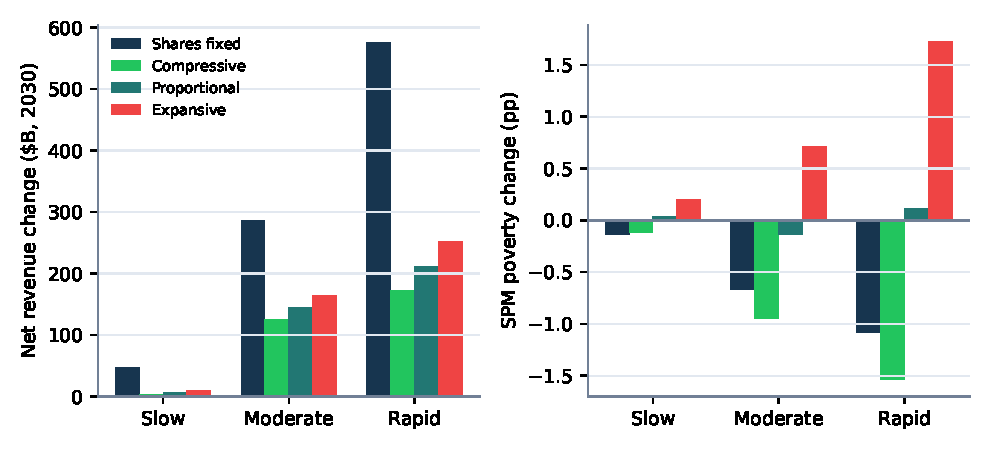
\includegraphics[width=0.95\textwidth]{figures/scenarios.pdf}
\caption{Net revenue (left) and SPM poverty change (right) by scenario and
wage-inequality variant, 2030.}
\label{fig:scenarios}
\end{figure}

The payroll-cap mechanism runs in both directions, which is worth stating
because it is easy to get backwards: under Rapid~/~compressive, aggregate
labor income \emph{falls} \genRapidCompLaborPct\% and payroll receipts still
\emph{rise} \genRapidCompPayroll B, because compression moves earnings from
above the taxable maximum to below it; under expansive the same cap turns
wage growth into a payroll loss of \genRapidExpPayroll B. The wage-spread
parameter also has a direct household reading: each variant has a crossover
wage below which workers lose (expansive,
\$\genRapidExpCrossover{}) or gain (compressive,
\$\genRapidCompCrossover{}), so under Rapid~/~expansive the great majority of
workers sit on the losing side of a scenario that adds \genRapidExpRev B to
net revenue.

\subsection{The transfer system}\label{sec:transfers}

The Revenue column of Table~\ref{tab:grid} nets transfers out; pulling them
apart shows the safety net responding exactly as designed
(Figure~\ref{fig:transfers}). Across the Rapid wage-spread variants ---
identical aggregate labor income, only its distribution varies --- gross tax
collections swing \$\genGrossTaxSwing B, and automatic transfer responses
absorb \$\genTransferSwing B of that swing, \genTransferAbsorbPct\%.
Non-credit transfers alone swing \$\genBenefitSwing B: \genRapidCompBenefits
B under compressive, as rising low-end wages float households off
means-tested programs, to \genRapidExpBenefits B under expansive as falling
ones push them on. SNAP carries \$\genSnapSwing B of the swing
(\genRapidCompSnap B to \genRapidExpSnap B) and SSI \$\genSsiSwing B;
Moderate shows the same shape (\genModCompBenefits B to \genModExpBenefits
B). Refundable credits contribute the remaining \$\genCreditSwing B --- a
response the Budget Lab's accounting does capture through its tax-credit
outlays line. The \$\genBenefitSwing B of program spending is the piece
outside their model's coverage, and it is the outlay side of the
\genRapidPovSpanPp pp poverty span: the same variant uncertainty their
report scores as a revenue question arrives at households as a benefits
question.

\begin{figure}[t]
\centering
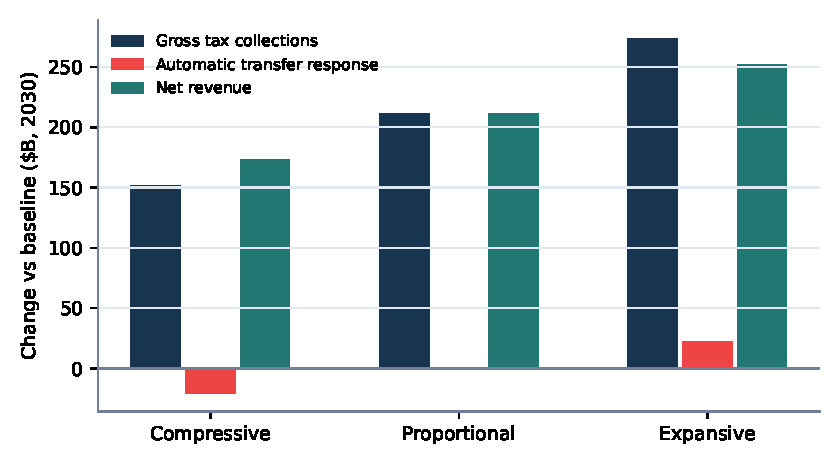
\includegraphics[width=0.8\textwidth]{figures/transfers.pdf}
\caption{Gross tax collections, automatic transfer response, and net revenue
across the Rapid wage-inequality variants, 2030. Transfers (refundable
credits plus benefits) rise exactly when workers lose, absorbing
\genTransferAbsorbPct\% of the gross-tax swing across the variants.}
\label{fig:transfers}
\end{figure}

\subsection{States}\label{sec:states}

State codes are the other channel a federal model does not carry. Under
Rapid~/~proportional they collect \genRapidPropState B, and the state take
doubles across the wage-spread variants (\genRapidCompState B to
\genRapidExpState B) as progressive state schedules concentrate collections
at the top the way federal brackets do. On the Rapid~/~expansive cell used
for the reconciliation below, state tax net of refundable state credits adds
\genRapidExpStateNet B --- roughly a sixth on top of the bridged federal
take.

The geography is concentrated (Figure~\ref{fig:states}): the top five states
collect \genStateTopFiveSharePct\% of the national state take
(\genStateFirst, \genStateSecond, \genStateThird, \genStateFourth,
\genStateFifth, in \$B). \genNZeroStates{} states collect exactly nothing
from the capital shock --- \genZeroStatesList{} --- and Washington is the
instructive exception: it has no income tax either, but its capital-gains excise tax
collects \genWAState B, more than the seven zero-collecting states combined.
A state that taxes capital gains participates in an AI capital boom; a state
that taxes only wages does not participate in an economy where wages are the
shrinking share. State-funded benefit responses are negligible in these runs
(the model's state-benefit registry at version \genModelVersion{} covers
state SSI supplements and child-care subsidies), so the automatic-stabilizer
response above is almost entirely federal. Sub-national cells this small
carry material data-calibration sensitivity --- Section~\ref{sec:stability}
shows a single data-build revision moving New York's take from
\$\genStabNYOld B to \$\genStabNYNew B --- so the state figures locate the
pattern rather than measure any one state precisely.

\begin{figure}[t]
\centering
\includegraphics[width=0.8\textwidth]{figures/states.pdf}
\caption{Top ten states by net state revenue change, Rapid~/~proportional,
2030.}
\label{fig:states}
\end{figure}

\section{The two assumptions that dominate}\label{sec:sensitivity}

\subsection{Realization}\label{sec:realization}

The Budget Lab's capital shock assumes AI leaves the realized share of
capital income unchanged, and they flag the assumption as a limitation.
It carries real weight: unrealized gains, retained earnings and accruals
inside retirement accounts never reach the individual tax base. Holding
Rapid~/~proportional fixed and varying only how much of the incremental
capital flow lands on a tax return (Figure~\ref{fig:realization},
Table~\ref{tab:realization} in the appendix), revenue runs from
\genRealZeroRev B at a 0\% realized share to \genRealFullRev B at their
100\% assumption --- linear to within a percent across a grid in
\genRealGridStepPct-point steps, with breakeven interpolated at a
\genRealBreakevenPct\% realized share (the grid's own adjacent points are
\genRealZeroRev B at 0\% and \genRealQuarterRev B at
\genRealGridStepPct\%). Below that, the household side of the fiscal system
loses money on Rapid AI growth: labor income still falls, and not enough
taxable capital income reaches returns to offset it.

One counterweight sits outside the household sector: corporate tax is levied
upstream of household realization, so the Budget Lab's corporate wedge would
still collect about \genTheirRapidCit B on the same shock regardless of the
realized share --- enough to keep the all-in total (household, state and
corporate) positive, about \genRealZeroAllIn B, even at the 0\% floor. Low
realization shifts the fiscal burden of an AI boom onto the corporate side;
it does not eliminate it. One scope note: the realization haircut applies
uniformly to all nine capital variables, including pass-through income and
retirement distributions that are realized by construction, so the low end
of the axis is a stress bound rather than a describable world.

Poverty is flat across the entire sweep, between \genRealPovMinPct\% and
\genRealPovMaxPct\%. Whether AI's capital gains are taxable moves the
federal balance sheet by more than a quarter-trillion dollars and moves poor
households essentially not at all: the transfer system responds to what
happens to wages, not to how much of the capital gain the tax system
reaches.

\begin{figure}[t]
\centering
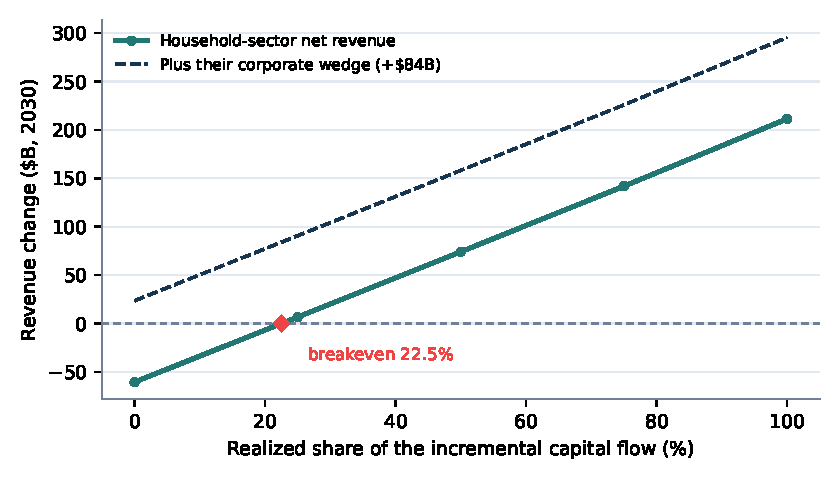
\includegraphics[width=0.8\textwidth]{figures/realization.pdf}
\caption{Net revenue under Rapid~/~proportional as the realized share of the
incremental capital flow varies. The dashed line adds the Budget Lab's
realization-independent corporate wedge.}
\label{fig:realization}
\end{figure}

\subsection{What counts as capital}\label{sec:scope}

Taxable pension and IRA distributions are taxed at ordinary rates. Counting
them in the capital set --- which the Budget Lab does, and the headline
results follow --- raises the revenue estimate and softens the ``capital is
taxed lightly'' mechanism. Excluding them (Table~\ref{tab:scope} in the
appendix) moves Rapid from \genRapidScopeFull B to \genRapidScopeExcl B and
flips Slow's sign (\genSlowScopeFull B to \genSlowScopeExcl B). Together
with realization, these two definitional choices span more of the revenue
answer than the choice between Slow, Moderate and Rapid.

\subsection{Stability across data builds}\label{sec:stability}

The results were first computed on the prior \texttt{populace-us} build
(build~o, 22 July 2026) and rerun on build~p (\genDataBuildDate{}, with
revised capital gains calibration) under the identical pinned model version
--- a data-only change. Both runs predate the Head Start correction noted
before the introduction, so this comparison uses the net-income accounting they
shared. No scenario revenue figure moved by more than
\$\genStabMaxAbsRevB B in absolute terms; in relative terms Moderate and
Rapid cells moved by at most \genStabMaxRelModRapidPct\%, while the smallest
Slow cells --- single-digit-billion bases --- moved by up to
\genStabMaxRelPct\%. Every poverty change moved by less than
\genStabMaxPovChangePp\,pp, and no conclusion changed. The recalibration's
visible effect is distributional: the baseline top-1\% net income share
rises from \genStabTopOneOld\% to \genStabTopOneNew\% (\genBaselineTopOnePct\%
after the correction), and New York's state
take under Rapid rises from \$\genStabNYOld B to \$\genStabNYNew B as more
of the gains land where they are taxed. This build-to-build movement bounds
sensitivity to data calibration, not sampling error, which is unquantified
here (Section~\ref{sec:discussion}). An average-tax-rate cross-check also
lands in range: Rapid~/~proportional turns a \genRapidPropMarketDelta B
market income increase into \genRapidPropRev B of receipts,
\genRapidPropATRPct\% --- of the same order as the 21--34\% band the Budget
Lab reports, though their denominator is gross factor income rather than
modelled market income.

\section{Reconciliation with the Budget Lab}\label{sec:reconciliation}

The two models measure different totals: theirs is federal individual income
tax plus payroll plus a corporate wedge, with no states and no non-credit
transfers; this paper's household total spans federal and state and nets out
refundable credits and the benefit programs counted in household net income,
a set that excludes health programs, Head Start and Early Head Start
(Section~\ref{sec:method}). Setting the headline numbers side by side without
a bridge would be wrong, so this section builds one, using only this paper's
run output and objects they publish. Their repository commits the complete
published result grid --- revenue by instrument for all eighteen cells ---
which makes the comparison possible at the cell level rather than against
two text-stated totals.

\textbf{Basis.} Their microsimulation total is individual income tax plus
payroll minus tax-credit outlays; the matching quantity here is federal
income tax net of refundable credits, plus payroll (both halves and
self-employment). Their corporate wedge reduces to the capital growth rate
times CBO's 2030 corporate anchor of \$486B --- in their formula
$\Delta R_{\mathrm{CIT}} = X \cdot (R_{\mathrm{CIT}}/Y^0_K)$ with
$X = Y^0_K\,g$, the capital base cancels --- and all \genTheirNCells{}
committed values equal $g \times \$486\mathrm{B}$ to within
\$\genCitWedgeMaxDevB B, checked against their own per-cell capital growth
rates. Adding their wedge
to this paper's federal microsimulation total yields a like-for-like
``bridged'' headline. The wedge is not PolicyEngine modelling corporate tax,
and it inherits every constant-rate assumption they list.

\begin{table}[t]
\centering
\tabBridge
\caption{The bridged headline cell (Rapid~/~expansive, their central
published scenario), \$B, 2030. ``IIT (net)'' is individual income tax net
of refundable credits; the corporate wedge is theirs in both rows.}
\label{tab:bridge}
\end{table}

\textbf{Where the models agree.} Payroll responses agree closely in all nine
as-forecast cells --- the largest gap anywhere in the grid is
\$\genPayrollMaxCellGap B (Table~\ref{tab:cells}). Across the Rapid variants
ours run \genPayrollTripletOurs{} against theirs
\genPayrollTripletTheirs{} for compressive~/~proportional~/~expansive ---
two independent models putting similar wage distributions against the same
taxable maximum, including the sign reversal under compression. The tilt
ratios also line up once stated on the same basis: on their
federal-plus-corporate accounting, shares-fixed revenue exceeds as-forecast
revenue by
\genTiltOursMatchedSlow$\times$~/~\genTiltOursMatchedMod$\times$~/~\genTiltOursMatchedRapid$\times$
here against
\genTiltTheirsSlow$\times$~/~\genTiltTheirsMod$\times$~/~\genTiltTheirsRapid$\times$
in their grid for Slow~/~Moderate~/~Rapid --- agreement on the paper's
central mechanism, with the same ordering. (The household-total ratio for
Rapid is larger, \genTiltOursHouseholdRapid$\times$, mainly because the
household basis omits the corporate wedge: the wedge grows with the capital
shock, so it cushions the as-forecast denominator on the matched basis.
States and transfers raise the tilt's dollar cost but leave the ratio
essentially unchanged.) Their most extreme published comparison
reproduces in direction but not in magnitude: for Slow with compressive
inequality, their grid puts revenue \genSlowCompTheirsLowerPct\% below the
shares-and-distribution-unchanged counterfactual (their text states 82\%),
while this paper gets \genSlowCompOursLowerPct\%. Slow cells are
also the least stable in this model: Section~\ref{sec:stability} shows them
moving up to \genStabMaxRelPct\% on a data-build refresh alone, because
their bases are single-digit billions. The agreement to take seriously in
this scenario is the sign and the ordering, not the second digit.

\begin{table}[t]
\centering
\small
\tabPayrollCells
\caption{Cell-level comparison on the matched federal basis, all nine
as-forecast cells, \$B, 2030.}
\label{tab:cells}
\end{table}

\textbf{Where they diverge, and why.} The bridged headline is
\genBridgeOursTotal B against their \genBridgeTheirsTotal B ---
\genBridgeRatio$\times$, or \genBridgeOursCboPct\% against
\genBridgeTheirsCboPct\% of the CBO 2030 revenue baseline
(\$\genTheirCBORevB B, from their committed grid). The gap concentrates in
the income-tax response to the capital shock, and the absolute gap says so
more clearly than any ratio: it is nearly constant at
\genIITGapTriplet{}~\$B across the three Rapid wage-spread cells, exactly
what a divergence in the shared capital shock --- rather than in the varying
wage channel --- would produce. (In ratio terms:
\genIITRatioProp$\times$ theirs on the proportional cell, where the
wage-spread channel is neutral; \genIITRatio$\times$ on the expansive
bridge cell.) Three model differences point the same direction. First, the
realized-capital base: their committed cell parameters put their baseline
realized taxable capital base at \$\genTheirYZeroKT T, against
\$\genModelledCapitalShareT T here --- \genBaseGapPct\% larger. Second,
allocation: they distribute the incremental capital flow by SCF-imputed
total wealth; this paper distributes by existing realized capital income,
which they note is the more top-concentrated choice --- and
top-concentrated dollars face higher marginal rates. Third, retirement
routing: taxable pension and IRA distributions here scale with the capital
shock and are taxed at ordinary rates. The capital-scope sensitivity of
Section~\ref{sec:scope} shows that last channel alone is worth about
\$\genRapidScopeDiffAbs B in Rapid.

\section{Discussion}\label{sec:discussion}

\subsection{What the results say}

Three readings of the results bear directly on policy questions the AI-fiscal
conversation is starting to ask. First, the fiscal and household questions
decouple. Capital-side tax design (the realization margin) moves the budget
by hundreds of billions while leaving poverty untouched; the wage-side
distribution moves poverty by \genRapidPovSpanPp pp while net revenue stays
positive throughout. A revenue estimate, however good, is not a household
forecast. Second, the automatic stabilizers are already in the scenario
arithmetic: transfers absorb \genTransferAbsorbPct\% of the gross-tax swing
across the wage-spread variants, which means deficit projections that stop
at the tax code overstate how much the wage-distribution assumption matters
fiscally --- and understate the program-side costs when workers lose. Third,
the state layer is not a rounding error: \genRapidPropState B under
proportional Rapid growth, doubling across wage-spread variants,
concentrated in a handful of states, and available only to states whose
codes reach capital income at all.

\subsection{Limitations}

\textbf{No corporate sector.} PolicyEngine-US models households; the
corporate wedge in Section~\ref{sec:reconciliation} is borrowed from the
Budget Lab, not modelled.

\textbf{Static.} No labor supply, saving, avoidance or enforcement
responses on either side of the comparison.

\textbf{Apportionment is narrower than theirs.} The incremental capital flow
follows existing realized capital income; their SCF-wealth apportionment
reaches households that hold wealth but realize nothing. By their own
account the narrower base is more top-concentrated, so this choice
concentrates the shock more than theirs. The model carries household
balance-sheet variables (\texttt{net\_worth}, \texttt{stock\_assets}), so an
asset-based variant is feasible and is identified future work; the open
modelling question is which person and which income type receives the new
flow in a household that currently realizes none.

\textbf{Pass-through split is coarser than theirs.} Their active/passive-%
aware rule is approximated by a single rule because the microdata carries no
active/passive flag, under-assigning the passive portion to capital.

\textbf{National shares versus modelled shares.} Scenario calibration uses
national factor shares ($\theta^0_L = 0.5550$); observed taxable microdata
flows are more labor-weighted (\$\genModelledLaborShareT T labor against
\$\genModelledCapitalShareT T capital), because survey and tax data miss
unrealized gains, retained earnings and imputed returns. Growth rates from
national accounts are applied to observed taxable flows --- the same choice
the Budget Lab makes with the PUF --- and both baseline shares are reported
so the gap is visible rather than assumed away. One implication is worth
stating for the headline tilt result: under Rapid, the as-forecast scenario
raises modelled market income by \genRapidPropMarketDelta B while the
shares-fixed counterfactual raises it by \genRapidFixedMarketDelta B,
because much of the forecast capital growth accrues to income the taxable
microdata does not observe. The tilt's revenue cost therefore combines a
composition effect with growth landing outside the modelled base; the
realization sweep of Section~\ref{sec:realization} is the sensitivity that
spans this margin.

\textbf{No sampling uncertainty.} Estimates carry survey-sampling and
imputation error that is not quantified here. The build-to-build comparison
of Section~\ref{sec:stability} bounds sensitivity to data calibration ---
material for sub-national and program-level cells --- but not sampling
error; small cells such as individual state takes and single-program
responses should be read to the nearest billion, not the decimal shown.

\textbf{Anchored poverty, unequivalized Gini.} SPM thresholds do not respond
to the simulated distribution, so a fully relative poverty line would rise
with five years of above-baseline growth and show larger increases. The
Gini is household-level and unequivalized: changes are meaningful, levels
are not comparable to published equivalized series. Poverty levels sit above
the published Census SPM rate \citep{census2025} --- a known calibration gap
--- so every poverty figure is a change against a same-year baseline on
identical thresholds.

\textbf{No health-program response.} Medicaid, CHIP and ACA subsidies are
excluded from net-income accounting in these runs by the model's default
switch; the transfer responses reported here would not shrink, and could
grow, with that channel on --- but this paper does not measure it.

\subsection{Next steps}

The wage-inequality parameter $\lambda$ is a stylization with, as the Budget
Lab says plainly, little evidence behind its magnitude. The natural
replacement is measured occupation-level exposure
\citep{felten2021, eloundou2024}: distributing the labor shock by exposure
scores mapped to CPS occupations would make the implied $\lambda$ an output
rather than an input --- the design of the UK companion paper
\citep{ahmadi2026}, and the ``S1'' expansion the Budget Lab's methodology
names as planned future work. Asset-based capital apportionment and a
policy-response layer (recycling the net revenue gain into transfers to test
whether the receipts can hold the bottom of the distribution harmless) are
the other two identified extensions.

\subsection{Conclusion}

Whether AI pays for itself fiscally depends on where its income lands ---
between factors, across the wage distribution, and on or off the individual
tax base. Running forecaster-calibrated scenarios through the full United
States tax and transfer system, the tilt toward capital keeps
\genKeptMatchedRapidPct\% of the revenue that balanced growth would deliver
on the federal basis and \genKeptHouseholdRapidPct\% on the household basis
(states and transfers, no corporate wedge), and it turns growth's poverty
gain into a marginal loss; the wage-distribution assumption nobody can yet
pin down flips the household verdict while the revenue verdict stands; and
the channels a tax-only model omits --- automatic transfers and state codes
--- carry a material share of the response. Where this model and
the Budget Lab's overlap, they agree closely; where they diverge, the
anatomy is identifiable and mostly definitional. All of it is open:
anyone can rerun these scenarios, or score a different future against them.


\clearpage
\input{sections/references}
\clearpage
\appendix
\section{Additional tables}\label{app:tables}

\begin{table}[h]
\centering
\tabRealization
\caption{Net revenue under Rapid~/~proportional by realized share of the
incremental capital flow, \$B, 2030.}
\label{tab:realization}
\end{table}

\begin{table}[h]
\centering
\tabCapitalScope
\caption{Capital-scope sensitivity: net revenue with and without taxable
pension and IRA distributions in the capital set (proportional variants),
\$B, 2030.}
\label{tab:scope}
\end{table}

\begin{table}[h]
\centering
\tabStates
\caption{Top ten states by net state revenue change (state tax before
refundable credits minus refundable state credits), Rapid~/~proportional,
\$B, 2030.}
\label{tab:states}
\end{table}

\begin{table}[h]
\centering
\tabSweep
\caption{The mechanism sweep, \genSweepYear{}: net revenue, federal income
tax, SPM poverty and net Gini by share of labor income shifted to capital.}
\label{tab:sweep}
\end{table}

\clearpage
\section{Shock routing into the tax base}\label{app:routing}

Several shocked variables are aggregates rather than raw inputs, so the
implementation verifies that overriding them moves taxable income rather
than being recomputed away. Traced against the model's gross-income and
market-income source registries (\texttt{gov.irs.gross\_income.sources} and
\texttt{gov.household.market\_income\_sources} in policyengine-us
\genModelVersion{}):

\begin{table}[h]
\centering
\small
\begin{tabular}{lll}
\toprule
Shocked variable & Route into IRS gross income & Route into market income \\
\midrule
employment income & via employment income, net of & listed source \\
 & pre-tax contributions & \\
self-employment income & listed source & listed source \\
long/short-term capital gains & capital gains & capital gains \\
qualified/non-qualified dividends & ordinary dividend income & dividend income \\
taxable interest & listed source & interest income \\
rental income & listed source & listed source \\
partnership and S-corp income & listed source & listed source \\
taxable pension income & listed source & pension income \\
taxable IRA distributions & taxable retirement distributions & retirement distributions \\
\bottomrule
\end{tabular}
\caption{Every shocked variable reaches both the federal tax base and
household market income. Qualified and non-qualified dividends are the two
components of ordinary dividends; short- and long-term gains the two
components of capital gains; tax-exempt interest is deliberately outside the
shocked set.}
\label{tab:routing}
\end{table}

Because every shocked variable reaches household market income, the
net-income identity closes; the maximum residual across scenarios is
\$\genIdentityMaxResidual B, and the labor aggregate lands on its target to
within relative error \genLaborTargetMaxErr{}.

\clearpage
\section{Reproducibility}\label{app:repro}

Everything in this paper runs from open source against openly published
microdata:

\begin{itemize}
\item \textbf{Model:} policyengine-us \genModelVersion{} via policyengine.py
\genRunnerVersion{} (the runtime certifies the model--data pairing).
\item \textbf{Data:} \texttt{populace-us} certified build
\texttt{\genDataBuild}.
\item \textbf{Code:} \texttt{github.com/PolicyEngine/ai-inequality} ---
scenario engine in \texttt{analysis/ai\_scenarios.py}, runner in
\texttt{analysis/compute\_ai\_scenarios.py}, sweep in
\texttt{analysis/compute\_shift\_sweep.py}, reconciliation in
\texttt{analysis/reconcile\_budget\_lab.py}. Every number and table in this
paper is emitted from the run outputs by
\texttt{analysis/emit\_paper\_values.py}; figures by
\texttt{analysis/paper\_figures.py}.
\item \textbf{Their side:} the Budget Lab's \texttt{AI-Fiscal} repository
(MIT license) commits the complete published result grid
(\texttt{results/aggregates/ai\_fiscal\_publishable\_2030\_latest.xlsx});
the reconciliation reads it directly, and a copy is committed alongside this
paper's own run outputs so the bridge is reproducible without a network
fetch. Their PUF-based input microdata cannot be redistributed, so their
pipeline is readable but not rerunnable by third parties; this paper's is
both.
\item \textbf{Canonical run outputs:} \texttt{analysis/outputs/ai\_scenarios.json}
(build~p) is committed with three comparison files:
\texttt{ai\_scenarios\_buildp\_published.json} (build~p as first published,
with Head Start and Early Head Start in net income) and
\texttt{ai\_scenarios\_buildo.json} (build~o), the stability comparison of
Section~\ref{sec:stability}; and \texttt{transfer\_detail\_buildp\_published.json},
program-by-program benefit totals on the published runtime, the source of the
Head Start amounts in the correction note. Every value and table in this
paper regenerates from the repository alone --- the full simulation need only
be rerun to change a scenario, not to check a number.
\item \textbf{Interactive companion:}
\url{https://policyengine.org/us/ai-inequality/income-shift} (scenario
explorer) and \url{https://policyengine.org/us/ai-inequality/budget-lab}
(memo-length summary).
\end{itemize}

Calibration unit tests reproduce all nine of the Budget Lab's published
derived scenario values to within 0.005\,pp from the two recovered
constants ($G_{\mathrm{CBO}}=1.0976$, $\theta^0_L=0.5550$) and re-derive the
labor share by grid search. The scenario runner checkpoints per-scenario
results and is resumable; run logs and build-o archives are kept under
\texttt{analysis/outputs/}.


\end{document}
